\chapter{Introduzione}

\section{Le basi del machine learning}

\subsubsection{Gli ingredienti del machine learning:}

\begin{itemize}
  \item [$\Rightarrow$] \fancyglitter{Task}: specifica di cosa si vuole fare;
  \item [$\Rightarrow$] \fancyglitter{Modelli}: il modello matematico per affrontare un determinato task;
  \item [$\Rightarrow$] \fancyglitter{Features}: il modo con cui sono descritti gli esempi.
\end{itemize}

\nt{L'\fancyglitter{apprendimento automatico} ruota attorno all'idea di estrarre una regola generale per risolvere un problema a partire da problemi già risolti.}

\ex{Etichettatura delle email spam}{
  \begin{center}
    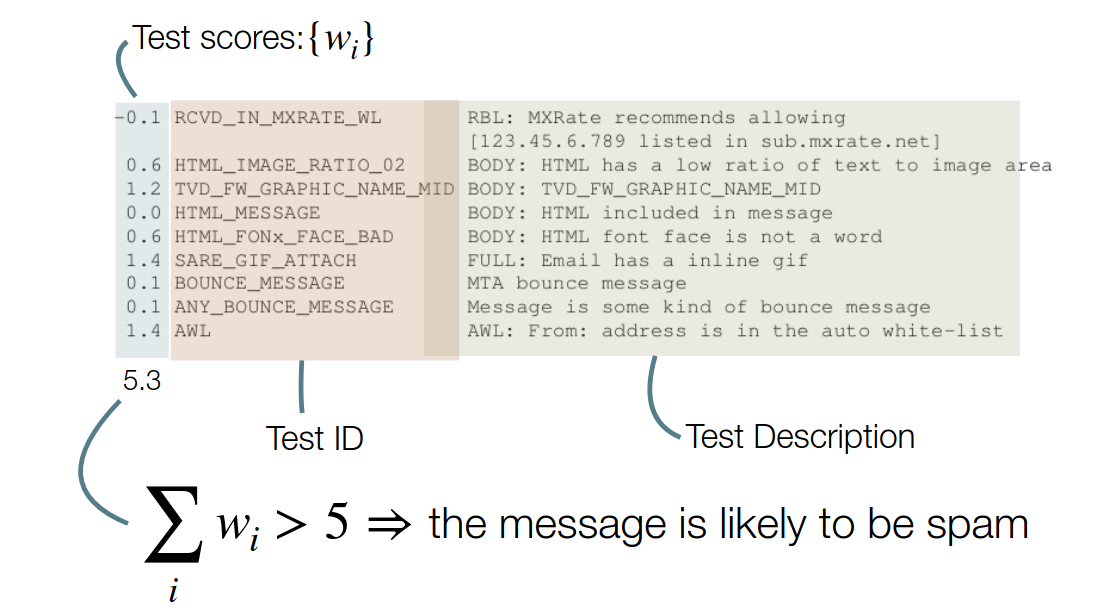
\includegraphics[scale=0.3]{01-Introduzione/Spam.png}
  \end{center}
  SpamAssassin è un filtro open-source usato per filtrare lo spam. Esso non lavora sul testo, ma su alcune \textit{feature} della mail. 
  \begin{center}
    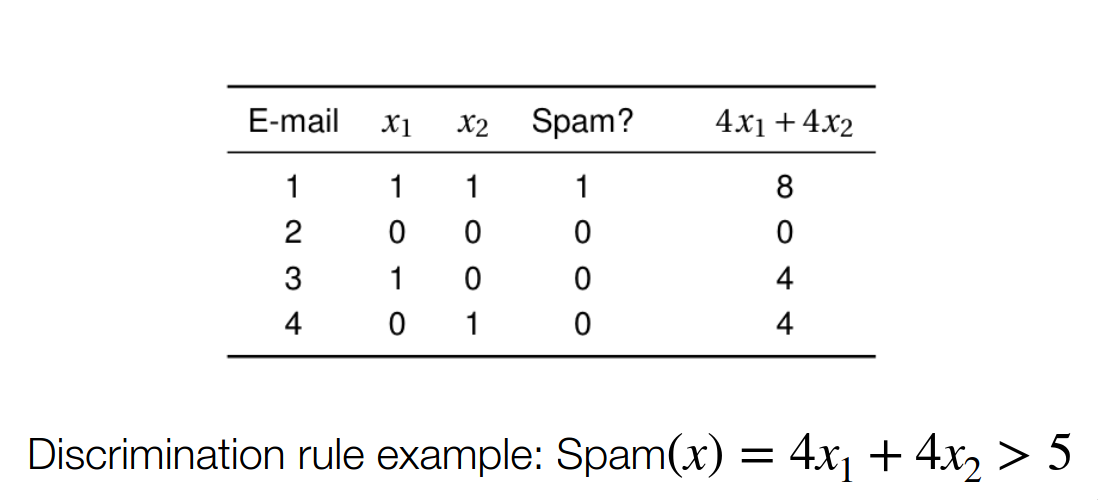
\includegraphics[scale=0.3]{01-Introduzione/Spam2.png}
  \end{center}
}

\dfn{Apprendimento automatico}{
  L'apprendimento automatico è lo studio sistematico di algoritmi e sistemi che migliorano le loro conoscenze e performance con l'esperienza.
}

